\documentclass[9pt, compress, xcolor=table]{beamer}


\usetheme{m}

\usepackage{amsmath,amssymb}
\usepackage{booktabs}
\usepackage[scale=2]{ccicons}
\usepackage{minted}
% \usepackage[utf8]{inputenc}
% \usepackage[T2A]{fontenc}
% \usepackage[english, russian]{babel}
%%% For accessing system, OTF and TTF fonts
%%% (would have been loaded by polylossia anyway)
\usepackage{fontspec}
%%% For language switching -- like babel, but for xelatex
\usepackage{polyglossia}
\setmainfont{PT Sans} % вообще шрифты определяются в теме бимера
\setmainlanguage{russian}
\setotherlanguages{english} %% or other languages

\usepackage{graphicx}
\usepackage{tabu} % https://ru.sharelatex.com/learn/Tables
\DeclareGraphicsExtensions{.pdf,.jpg,.png}
\graphicspath{{../images/}{./images/}}

\colorlet{Mycolor1}{green!50!blue!50!}

\usemintedstyle{trac}

\title{Физические принципы микроскопии сверхвысокого разрешения}
\subtitle{осенний семестр, 2018}
\author{ассистент, к.ф.-м.н. Шутова О.А.}
\institute{МГУ им. М.В. Ломоносова, физический факультет}

\begin{document}

\maketitle

\plain{}{Лекция 2. Свойства оптического ближнего поля}

\begin{frame}{Структура лекции и источники}
    
    \begin{itemize}
    \item Общие свойства оптических ближних полей.
    
    \item Зоны излучения гармонически колеблющегося диполя (L. Novotny, B.Hecht, II ed., Ch.8, p.234).
    
    \item Свойства излучения в закритической области (L. Novotny, B.Hecht, II ed., Ch.2, p.32).
    
    \item Перенос энергии эванесцентным полем. Нарушенное полное внутреннее отражение (ibid.).
    
    \item Силы, действующие на частицы в электромагнитном поле (A. Zayats, D. Richards, Ch.2,p. 22). 
    \item Частицы в эванесцентных полях: сдвиг, вращающий момент (серия работ Konstantin Bliokh "Mie scaterring and optical forces from evanescent fields", "Extraordinary momentum and spin in evanescent waves" et al.).
    \item Поляризационное состояние ближних полей, необходимость введения обобощенной сферы Пуанкаре (V. Zadkov, Yu. Vladimirova, et al.).
    
    \end{itemize}
    
\end{frame}

\section{Определение понятия и основные физические свойства}

\begin{frame}{Базовые свойства ближнего поля}

\begin{itemize}
\item Термин "<ближнее поле"> в оптику пришел из радиофизики (теории антенн)
\item Дальнее поле распространяется от излучающего объекта, и не воздействует (ни само, ни переизлученное) на свой источник, ближнее поле характеризуется влиянием эффектов (1) радиационного трения и (2) локального окружения
\item Индикатриса рассеяния в дальней зоне имеет вид восьмерки, перпендикулярной оси дипольного излучателя, в ближнем поле она наоборот вытянута вдоль этой оси
\item В дальней зоне количество энергии, проходящей через сферу, не зависит от расстояния, в ближнем поле происходит циркуляция энергии
\item Излучение гармонически колеблющегося диполя в дальнем поле характеризуется как поперечная ЭМ волна с линейной поляризацией, для ближнего поля мы должны вводить состояние поляризации посредством параметров Стокса
\end{itemize}


\end{frame}

\begin{frame}{Базовые свойства ближнего поля}

\begin{itemize}

\item Ближнее поле характерно наличием в нем неоднородных (эванесцентных) волн
\item Неоднородная волна отсутствует только в случае распространения плоской ЭМ волны в бесконечном однородном пространстве, любая граница раздела приводит к возникновению области ближнего поля
\item Объекты размером больше длины волны "<обтекаются"> светом по законам интерференции и дифракции в пределе Фраунгофера
\item Субволновые объекты выступают в качестве антенн для излучения, усиливая эффекты ближнего поля
\item Ближнее поле - это область порядка длины волны вокруг источника поля, дальнее поле (зона Фраунгофера) много больше длины волны, между ними присутствует зона промежуточного поля
\item В радиофизике ближнее поле делятся на реактивную зону (ближнюю к источнику) и излучательную зону (зону Френеля)

\end{itemize} 

\end{frame}

\begin{frame}{Поле гармонически осциллирующего диполя}

\begin{columns}[c]
\column{4.0cm}
\begin{center}
{\small Сферическая система координат}
\end{center}


\begin{center}
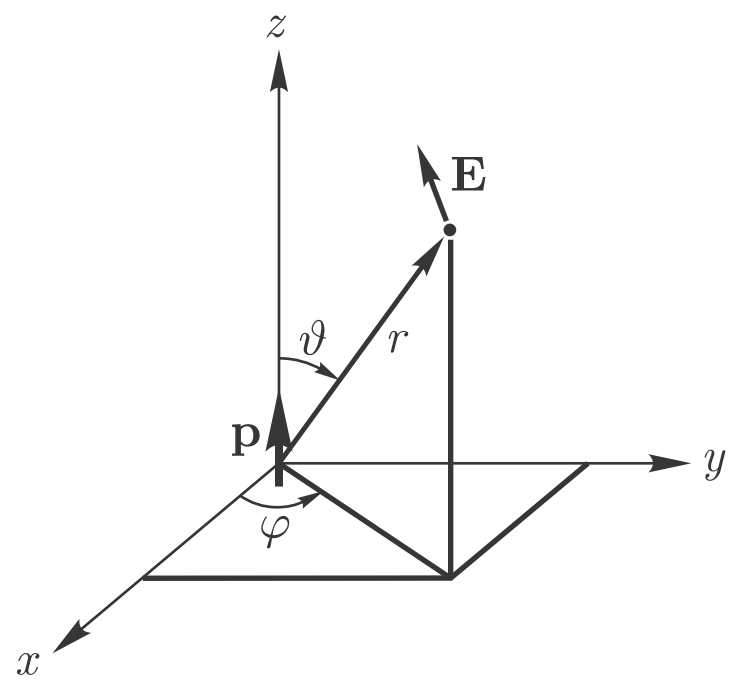
\includegraphics[scale=0.9]{SphericalCoordinates}
\end{center}
\begin{equation*}
\vec r=(r,\, \theta,\, \phi).
\end{equation*}

\column{7cm}

\begin{equation*}
p = \frac{p_0}{r} \exp \left[ \imath (kr - \omega t) \right]
\end{equation*}

\begin{equation*}
E_r = 2\cos\theta \cdot \left( \frac{1}{k^2r^2} - \frac{\imath}{kr} \right) k^2 p, 
\end{equation*}

\begin{equation*}
\quad E_{\theta} = \sin\theta \cdot \left( \frac{1}{k^2r^2} - \frac{\imath}{kr} - 1 \right) k^2 p,
\end{equation*}

\begin{equation*}
H_{\phi} = -\imath \sin\theta \cdot \left( \frac{1}{kr} - \imath \right) k^2 p, 
\end{equation*}

\begin{equation*}
E_{\phi} = H_r = H_{\theta} = 0,
\end{equation*}

Наличие компоненты поля $E_r$ является  характерной особенностью ближнего поля. Именно она нарушает пространственную поперечность ЭМ волны. Мы будем называть ее \textcolor{red}{продольной}. И часто будем бороться за ее увеличение.

\end{columns}

\end{frame}

\begin{frame}{Дефазировка электрической компоненты ближнего поля}

\begin{center}
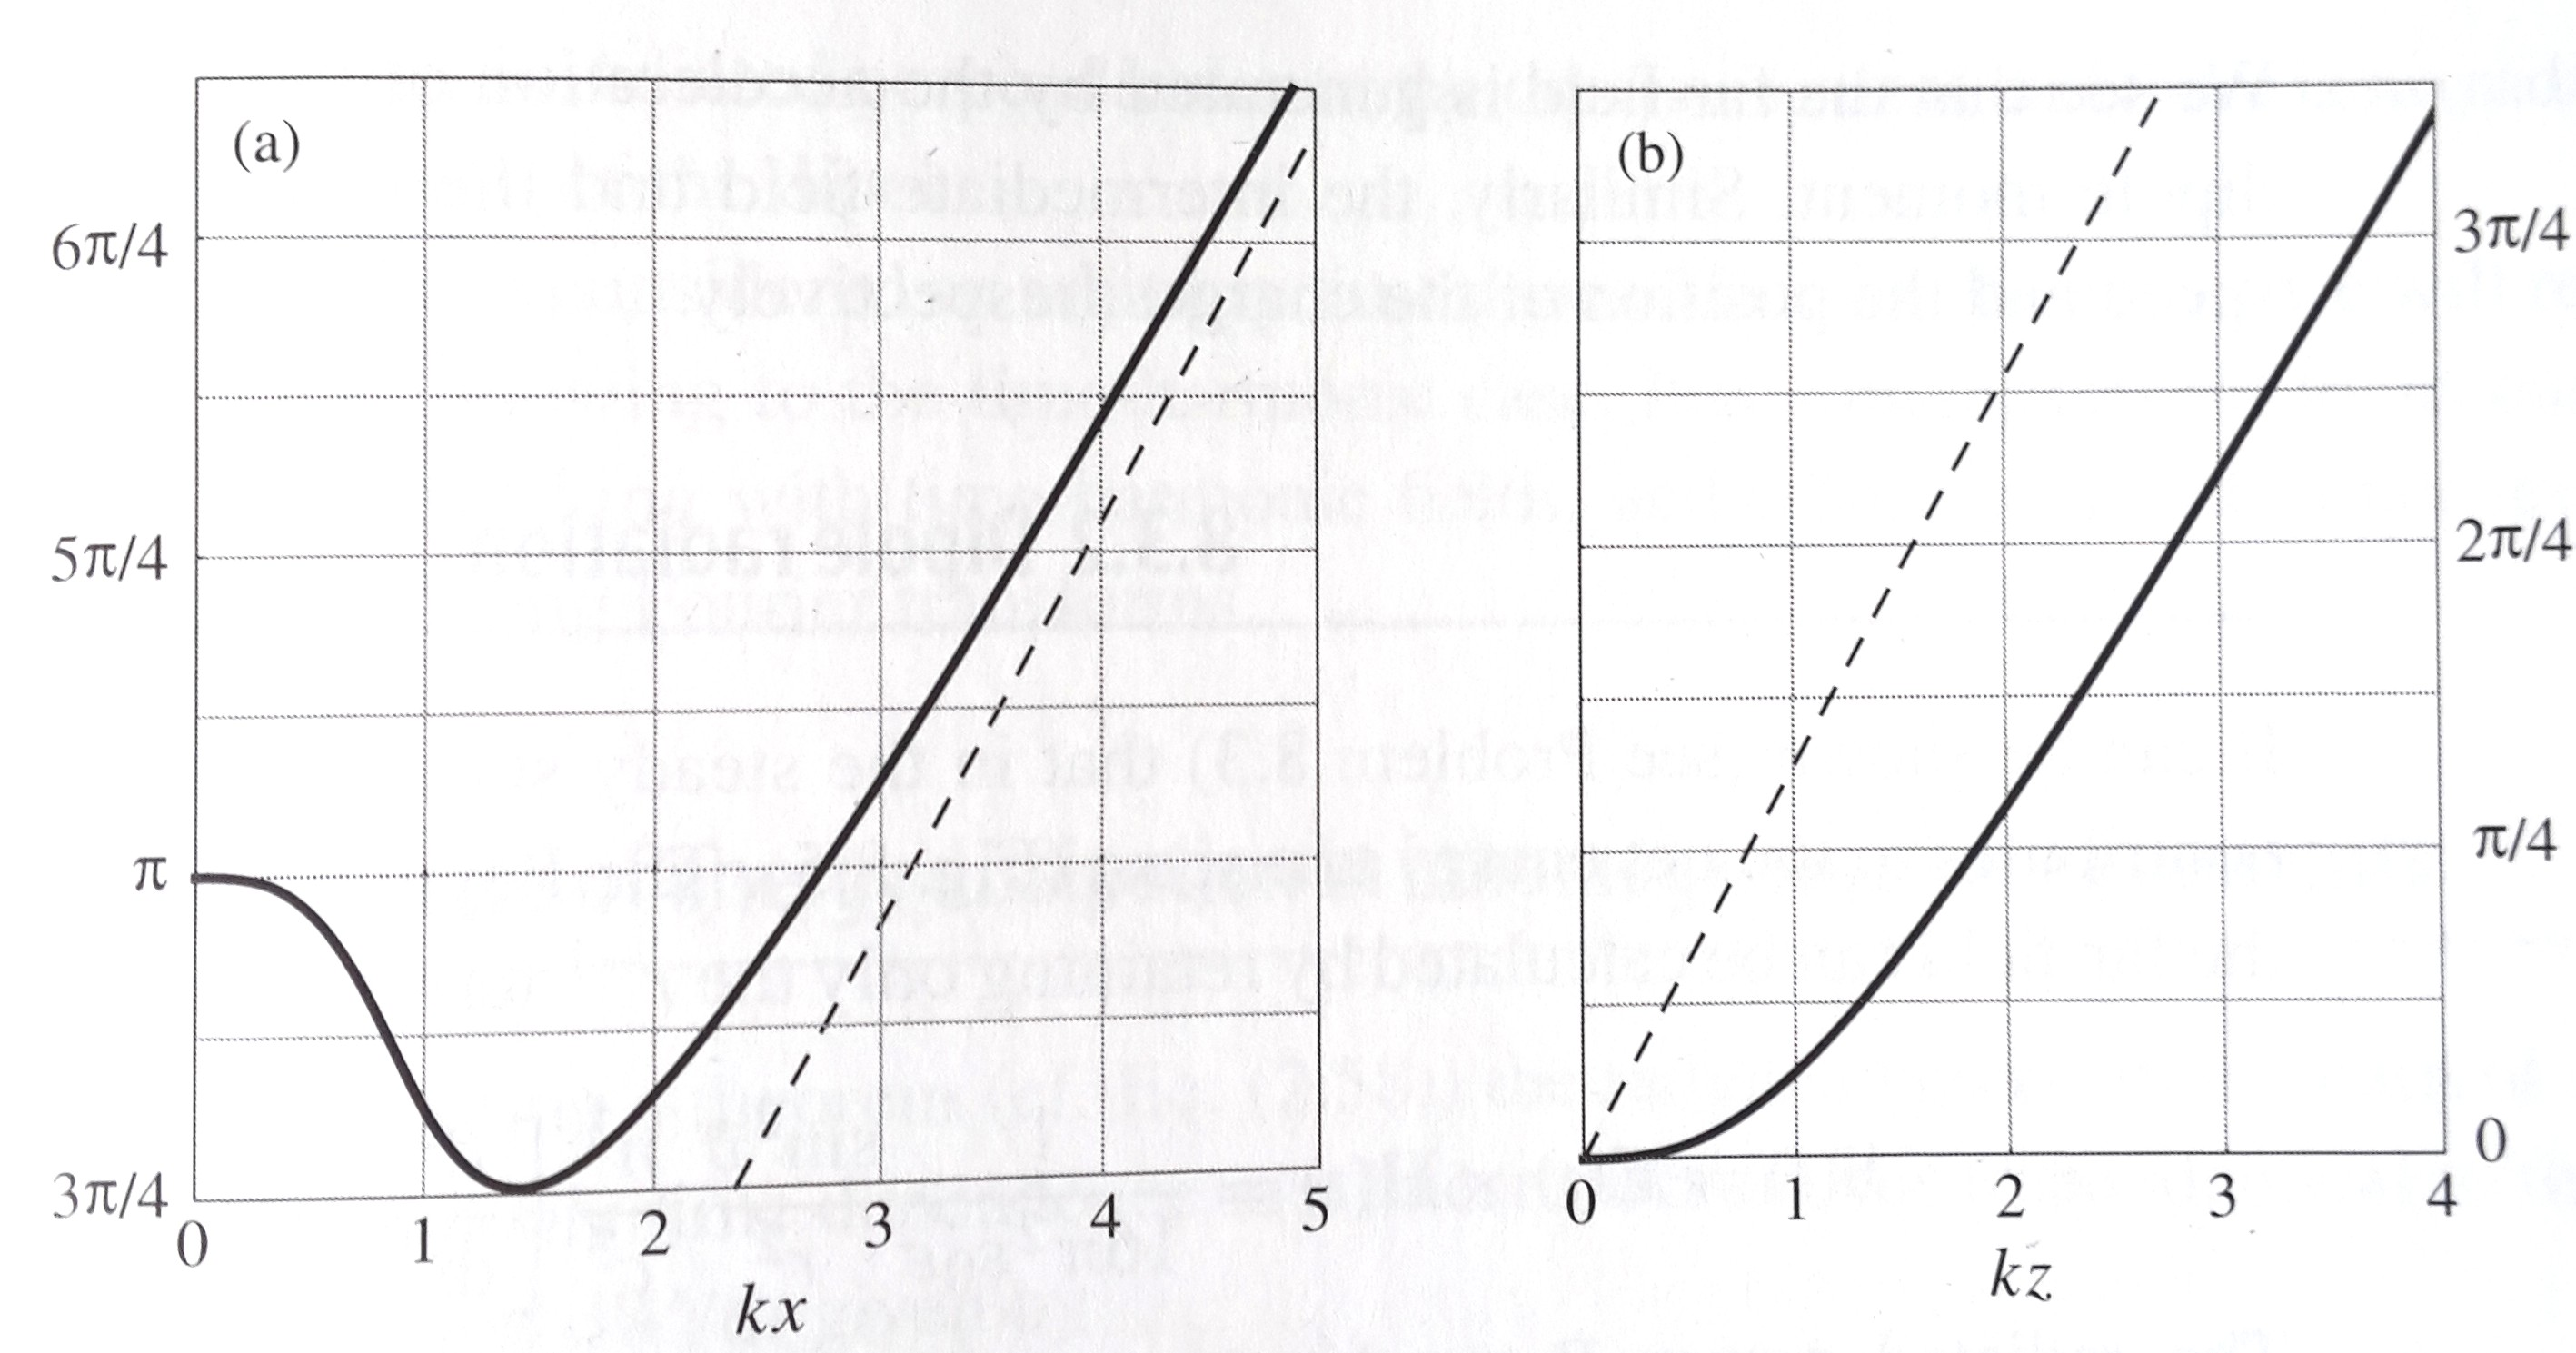
\includegraphics[width=0.8\textwidth]{phase1}
\end{center}

Слева: сдвиг фаз поперечной компоненты электрического поля по отношению к фазе колебаний диполя, рассчитанный вдоль оси $x$, в нуле в противофазе, затем выходит на фазу сферической волны;

Справа: сдвиг фаз продольной компоненты электрического поля по отношению к фазе колебаний диполя, рассчитанный вдоль оси $z$, в нуле синфазны, но на фазу сферической волны не выходит, достигая величины $90^{0}$.

\end{frame}


\begin{frame}{Дефазировка в области полного внутреннего отражения}

\begin{center}
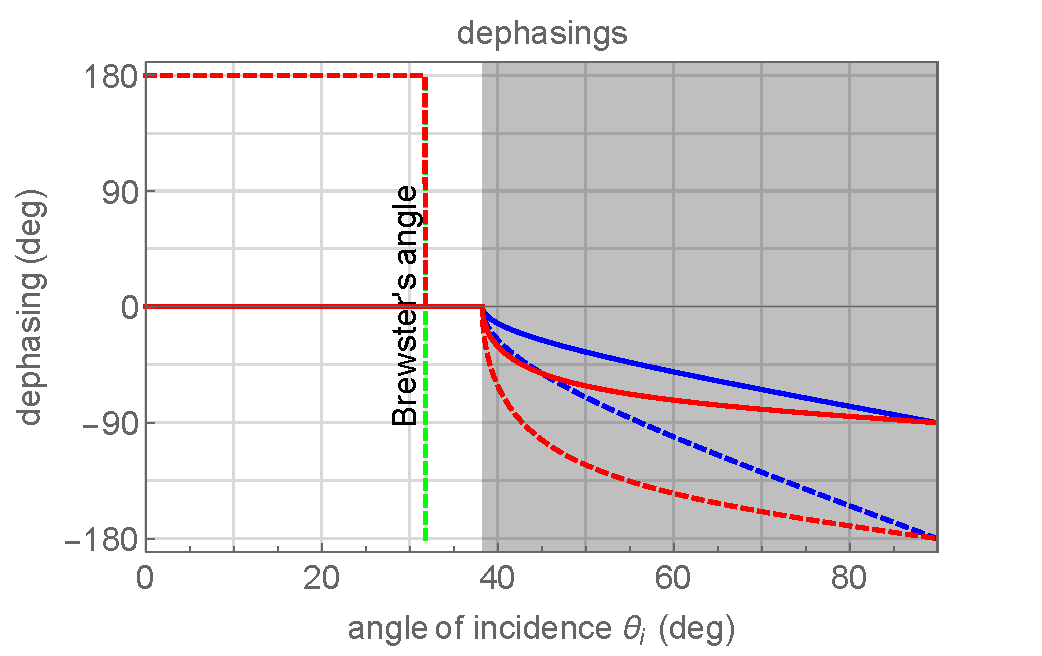
\includegraphics[width=0.8\textwidth]{fc_d}
\end{center}

Переход в область полного внутреннего отражения характеризуется формированием неоднородной волны у поверхности и увеличением расфазировки между падающей и отраженной и прошедшей волнами соответственно, причем для любой поляризации падающего излучения.


\end{frame}

\begin{frame}{Дипольное излучение}
\begin{equation*}
\label{eq_8.69}
\vec S(t)=\vec E(t)\times\vec H(t)=\frac{1}{16\pi^2\varepsilon_0\varepsilon}\frac{\sin^2{\theta}}{r^2}\frac{n^3}{c^3}\left[\dfrac{d^2}{dt^2}\left|\vec p\left(t-\frac{nr}{c}\right)\right|\right]^2\vec n_r.
\end{equation*}
\smallskip
\begin{equation*}
\label{eq_8.70}
P(t)=\int_{\Delta S}\vec S(t)\cdot\vec nds=\frac{1}{4\pi\varepsilon_0\varepsilon}\frac{2n^3}{3c^3}\left[\dfrac{d^2|\vec p(t)|}{dt^2}\right]^2,
\end{equation*}
\smallskip
\begin{equation*}
\label{eq_8.71}
\bar P=\frac{|\vec p|^2}{4\pi\varepsilon_0\varepsilon}\frac{n^3\omega^4}{3c^3}.
\end{equation*}
\smallskip
\begin{equation*}
\label{eq_8.72}
\frac{\bar P(\theta, \phi)}{\bar P}=\frac{3}{8\pi}\sin^2{\theta}.
\end{equation*}


\begin{columns}[c]

\column{4cm}

\centering
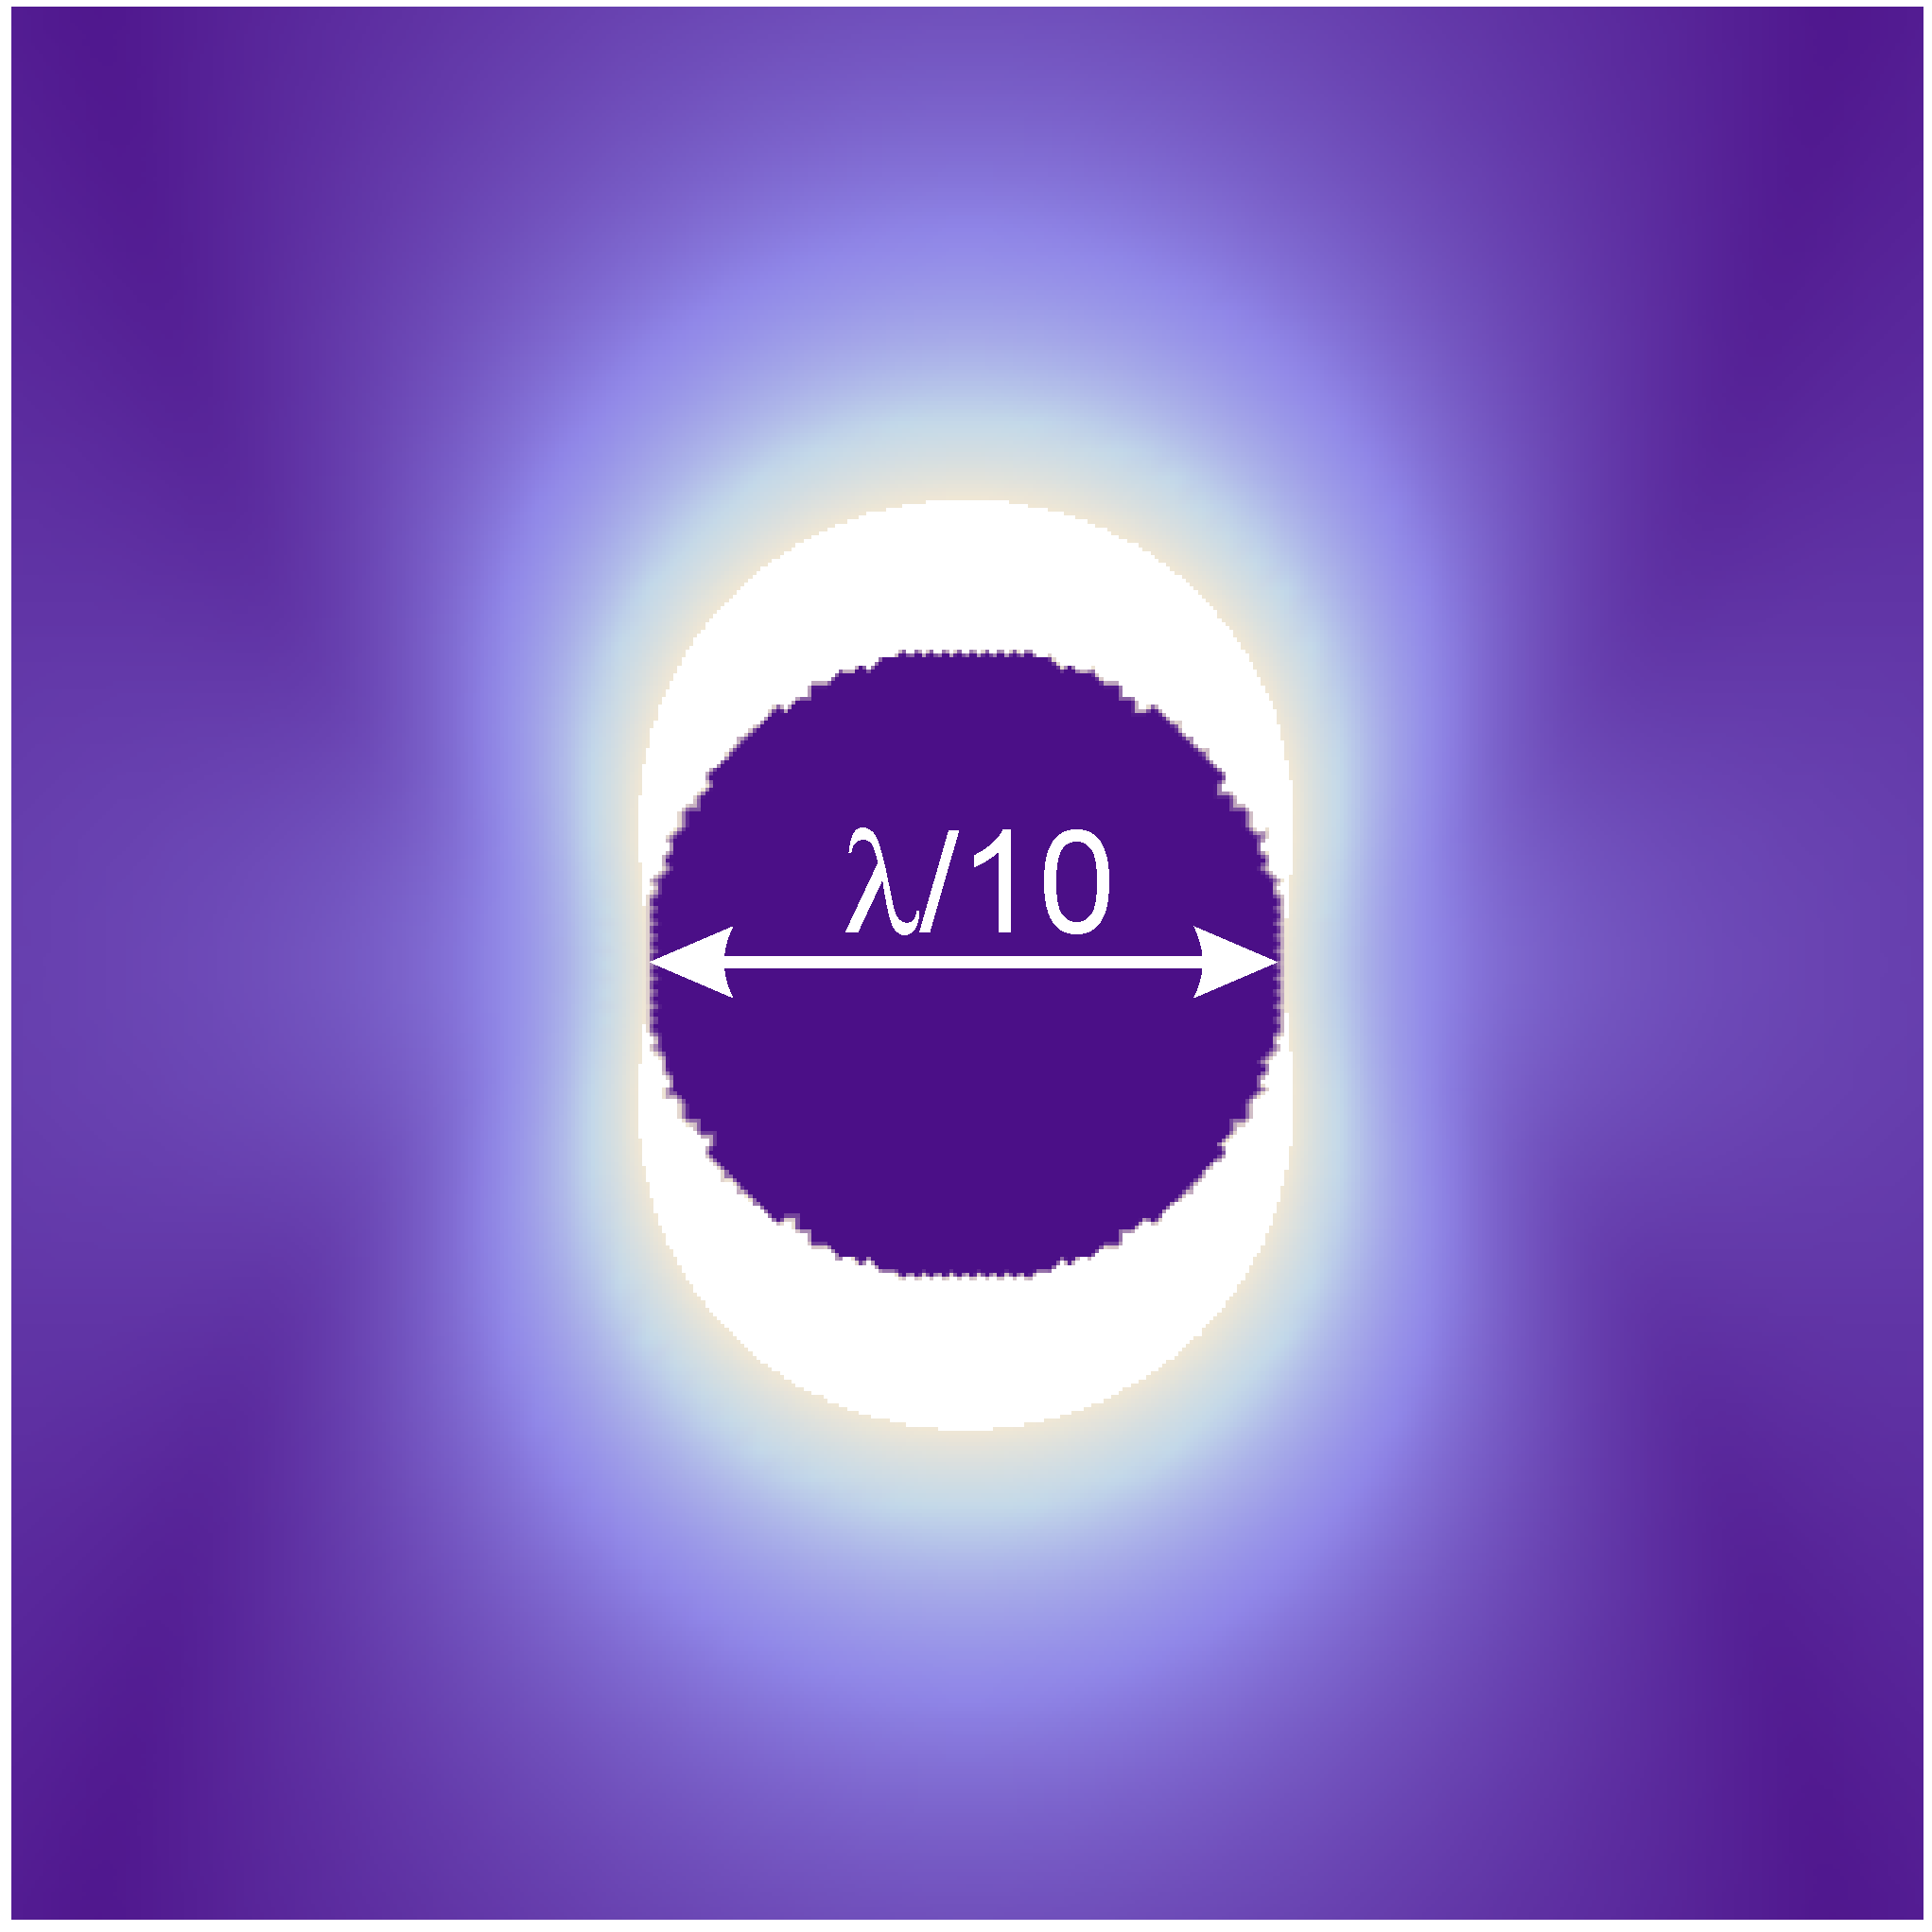
\includegraphics[width=0.9 \textwidth]{near}
\\\scriptsize{в ближнем поле}


\column{4cm}
\centering
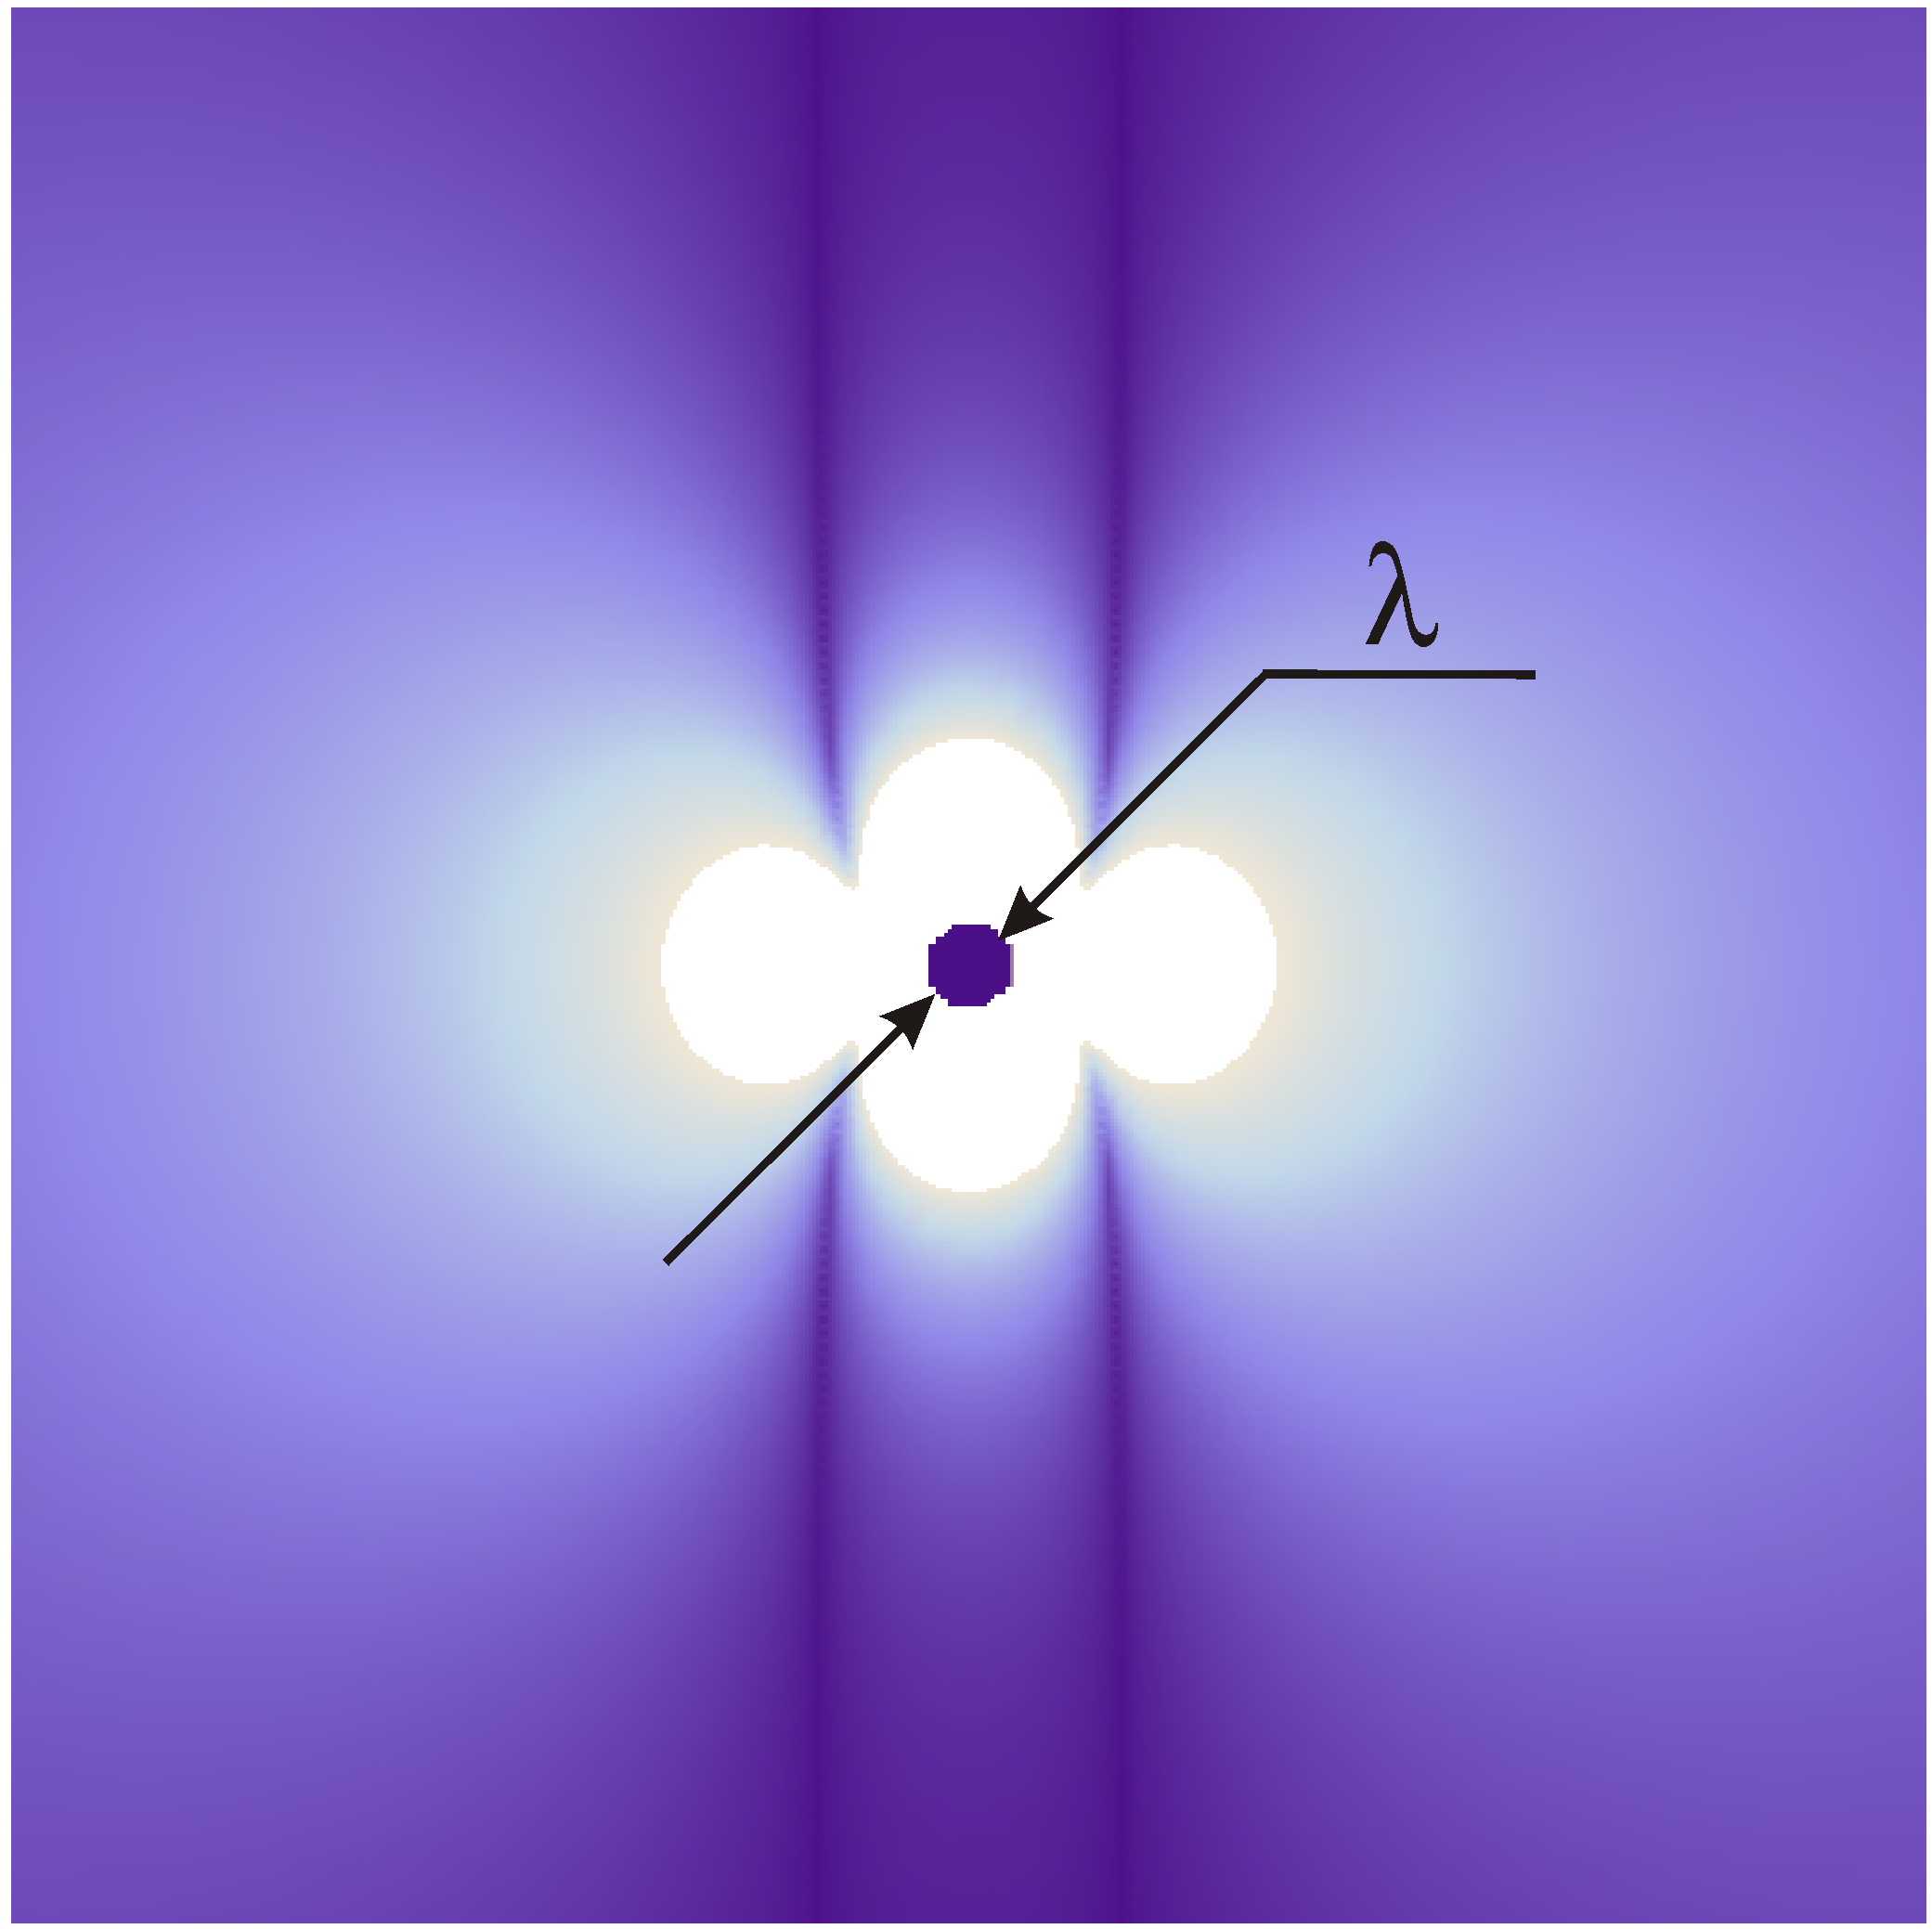
\includegraphics[width=0.9\textwidth]{mid}
\\\scriptsize{в промежуточном поле}

\column{4cm}
\centering
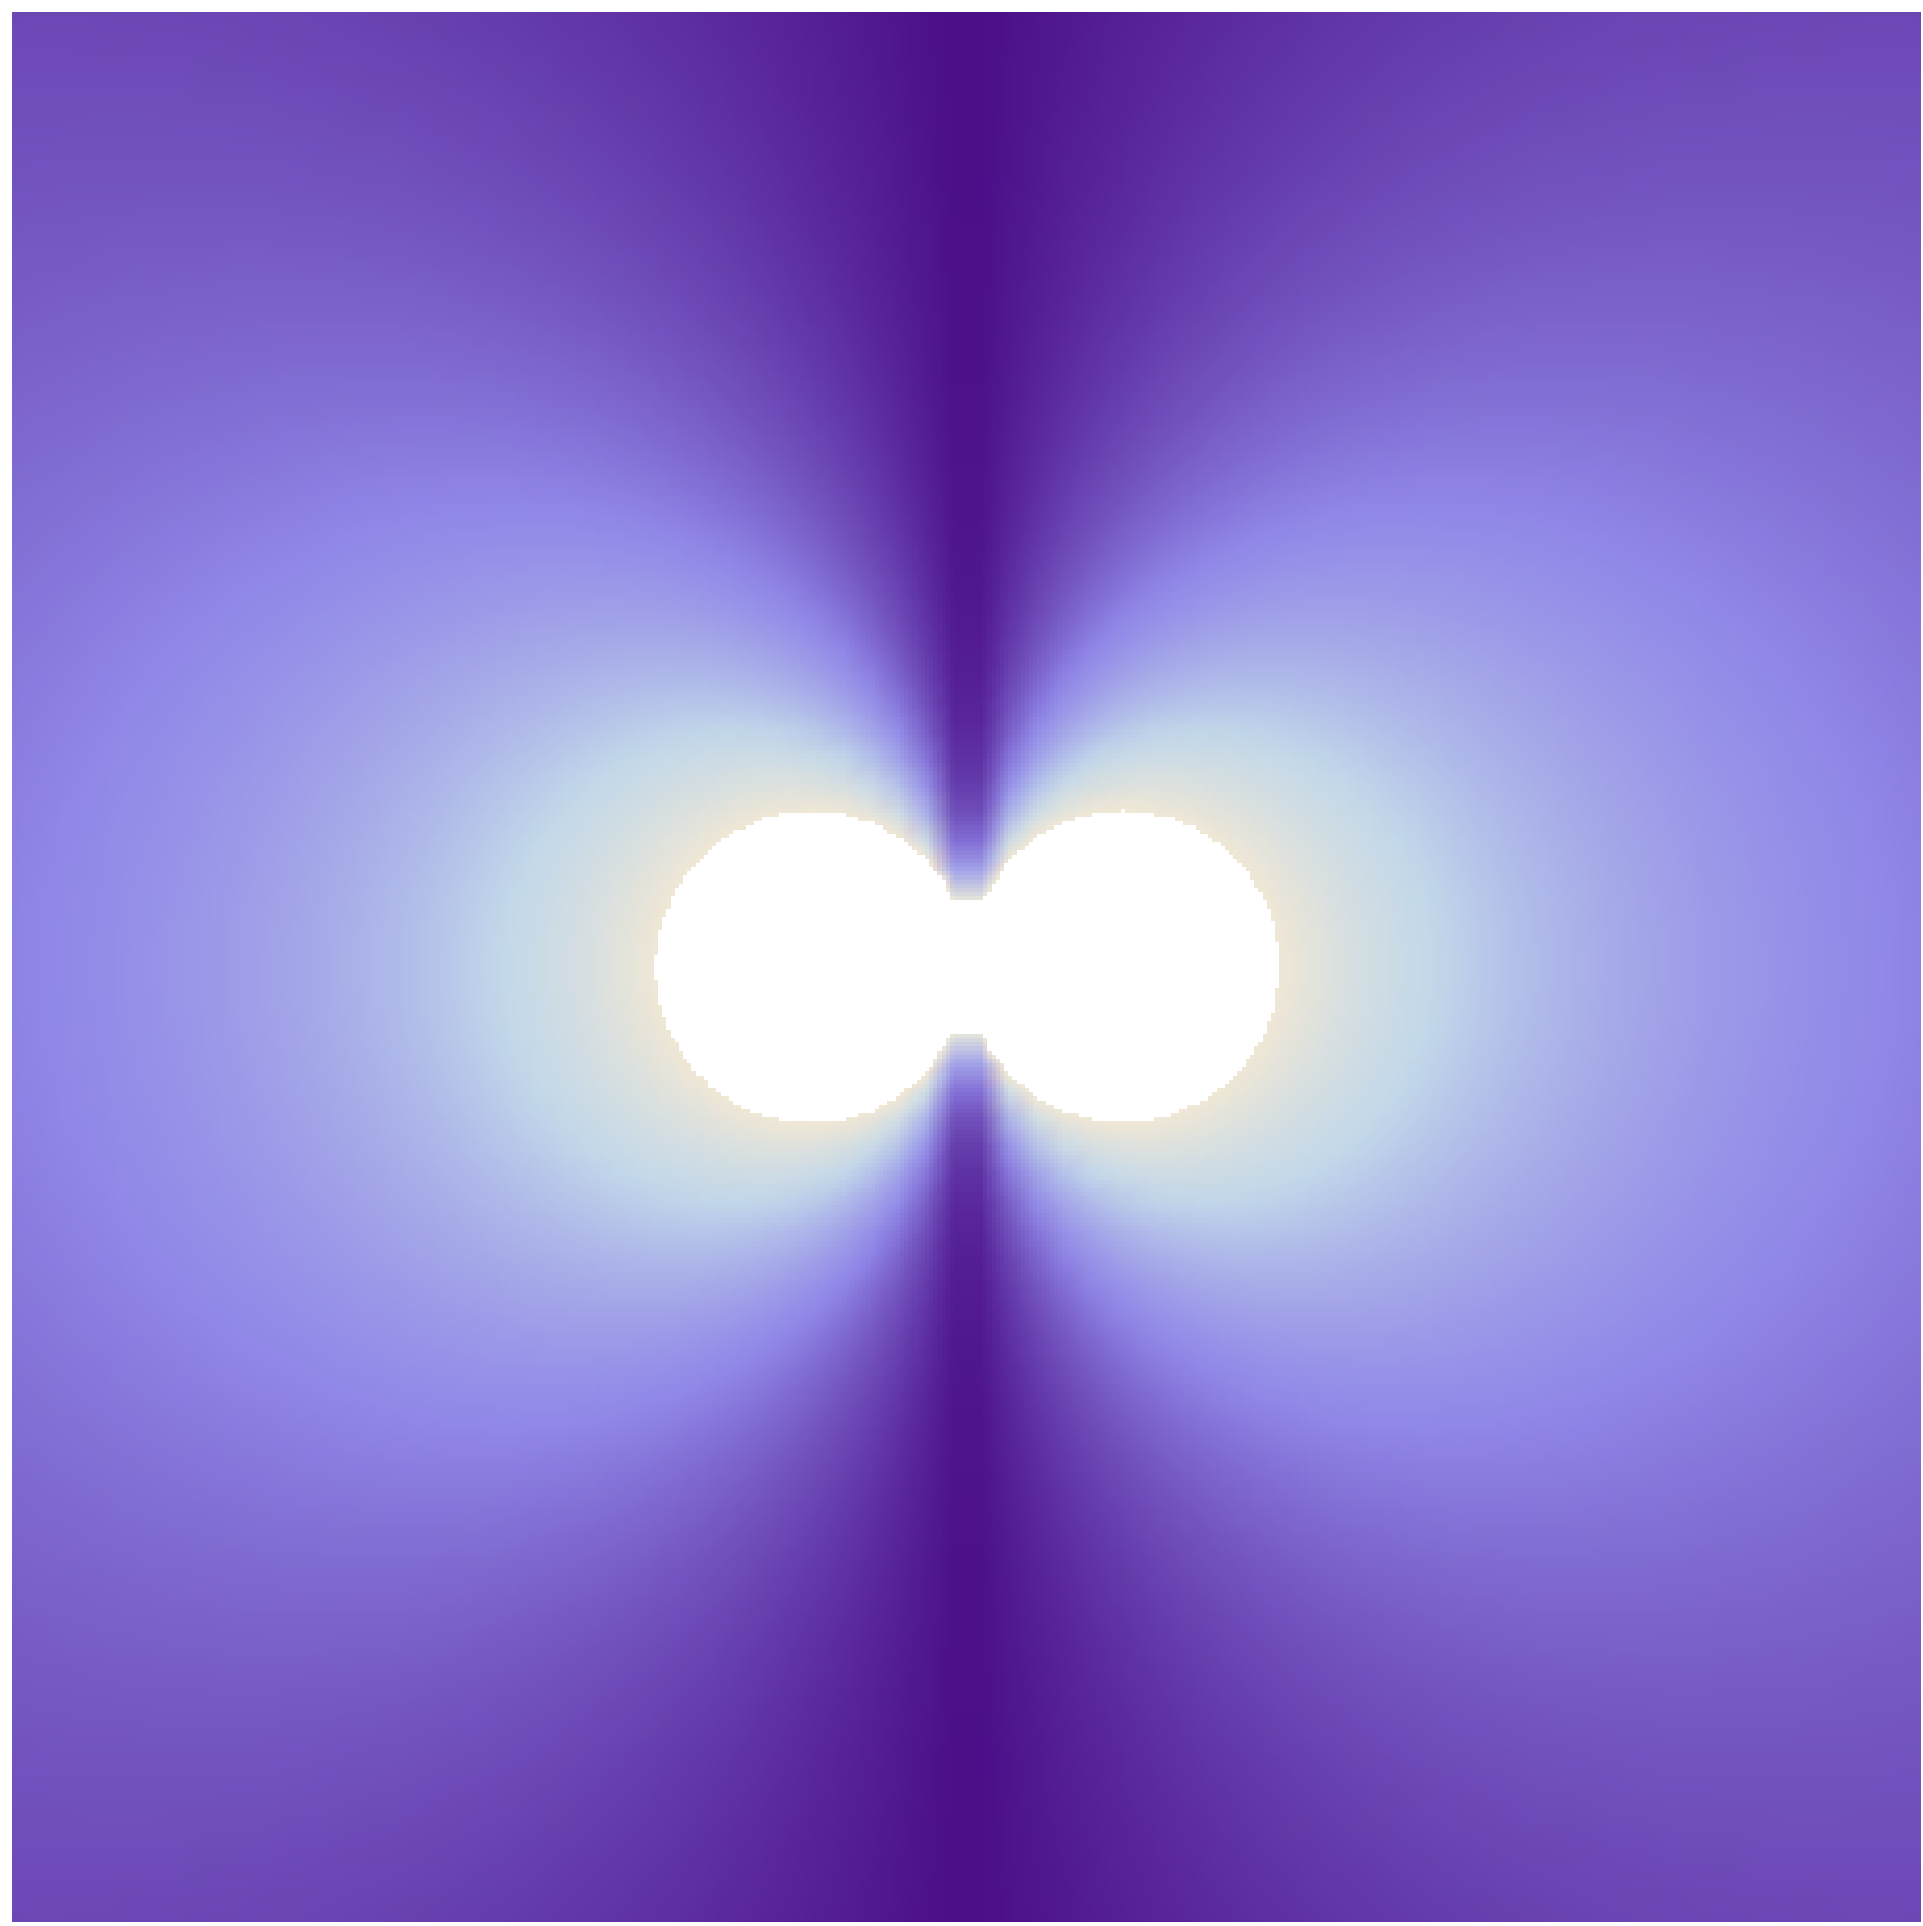
\includegraphics[width=0.9\textwidth]{far}
\\\scriptsize{в дальнем поле}


\end{columns}

\end{frame}



\begin{frame}{ПВО для разных поляризаций падающего поля}
\begin{center}
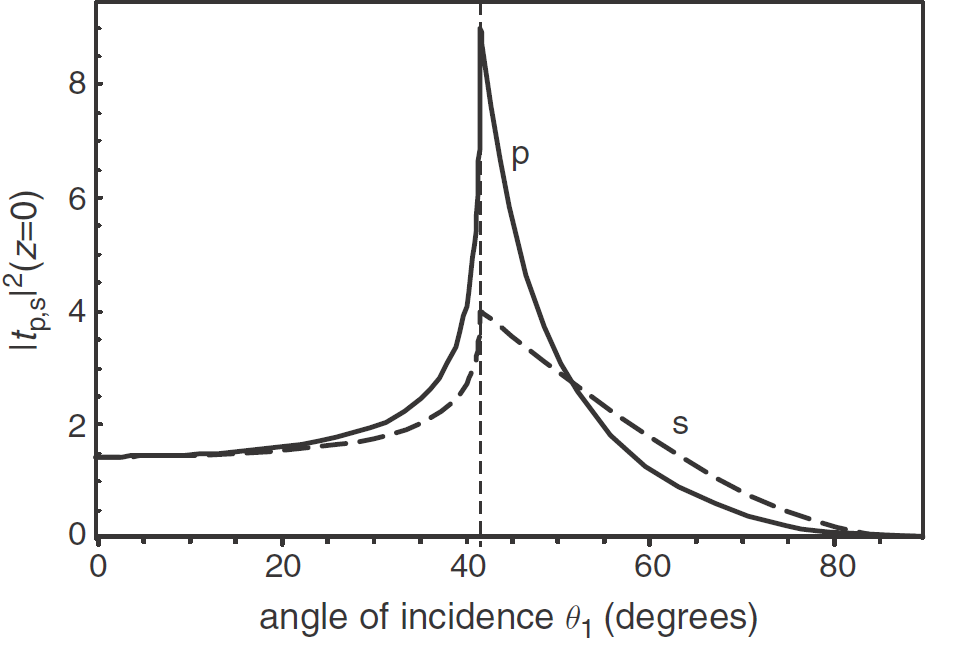
\includegraphics[width=0.7\textwidth]{ftir}
\end{center}

Обратим внимание, что интенсивность эванесцентного поля в непосредственной близости от границы может превышать интенсивность падающего поля в разы. Например, для границы воздух стекло: в 9 раз для p-поляризации и в 4 раза для s-поляризации.

\end{frame}

\begin{frame}{Угол максимальной перекачки энергии }
падающей волны в продольную волну
\begin{center}
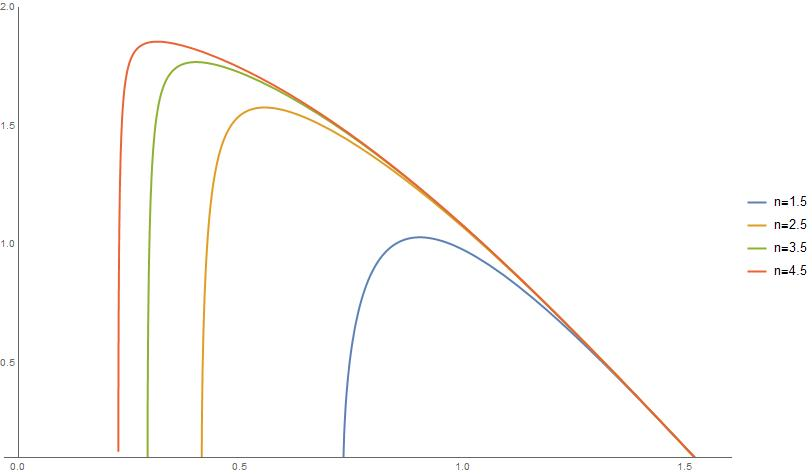
\includegraphics[width=0.9\textwidth]{fig.jpg}
\end{center}

Исследуем коэффициент связи между p-компонентой падающей волны и продольной эванесцентной волной во второй области $E_{x2}/E_{ip}$

\end{frame}

\begin{frame}{Вектор Умова-Пойтинга эванесцентной волны}
    
    \begin{columns}[c]

\column{6.5cm}

\begin{center}
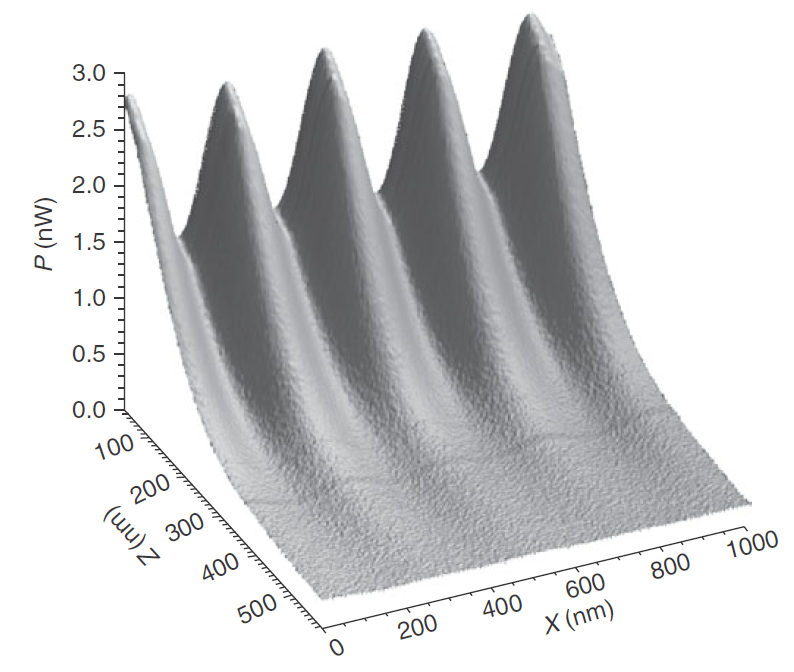
\includegraphics[width=0.9\textwidth]{stand}
\end{center}

Стоячая эванесцентная волна, возникающая в результате интерференции двух эванесцентных волн.

\column{6cm}

\textcolor{red!50!black}{Важно}: равенство "$1$" коэффициента отражения по интенсивности при ПВО не означает, что поток энергии во второй среде отсутствует.

\begin{multline*}
    \langle S\rangle_x=\frac{1}{2}\sqrt{\frac{\epsilon_2\mu_2}{\epsilon_1\mu_1}}\sin{\theta_1}\left(|t^s|^2|\vec E_1^{(s)}|^2 +\right.\\\left.+|t^p|^2|\vec E_1^{(p)}|^2 \right)e^{-\gamma z}
\end{multline*}

То есть эванесцентная волна переносит энергию вдоль поверхности в направлении поперечного волнового вектора $\vec k_{\perp}=\vec k_x+\vec k_y$
\end{columns}
\end{frame}

\begin{frame}{Нарушенное полное внутреннее отражение}

\begin{columns}[c]

\column{6.5cm}

\begin{center}
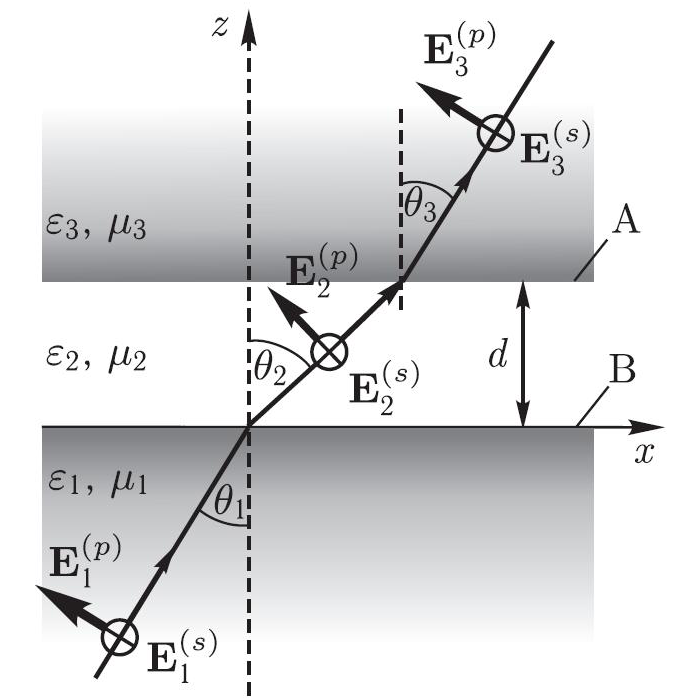
\includegraphics[width=0.9\textwidth]{fig2_05}
\end{center}

\column{6.5cm}
\begin{center}
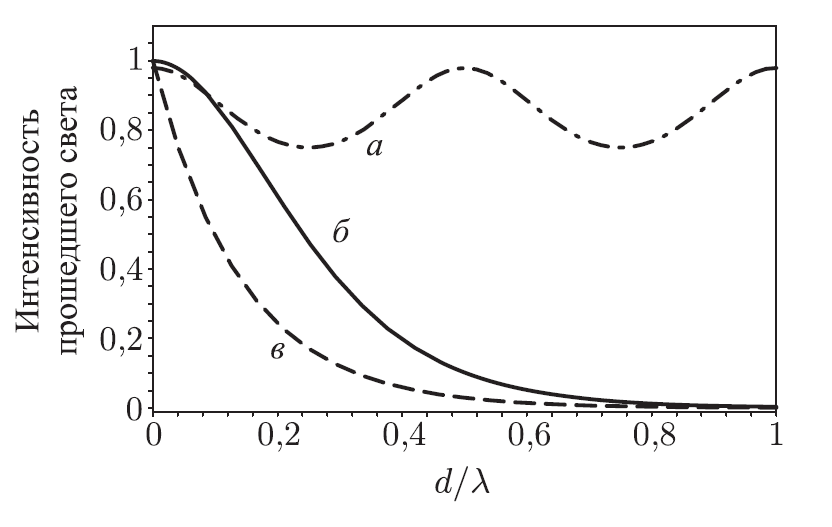
\includegraphics[width=0.9\textwidth]{fig2_14}
\end{center}

Кривая (б) есть сумма двух экспонент, затухающей и отраженной от второй границы: $c_1 e^{-\gamma z}+c_2 e^{+\gamma z}$ 

Три режима:
\begin{enumerate}
    \item $\theta_1<\text{arcsin}\frac{n_1}{n_2}$
    \item $\text{arcsin}\frac{n_1}{n_2}<\theta_1<\text{arcsin}\frac{n_3}{n_1}$ НПВО
    \item $\theta_1>\text{arcsin}\frac{n_3}{n_1}$ 
\end{enumerate}
\end{columns}
\end{frame}

\begin{frame}{Наиболее распространенные схемы}
по созданию и изучению ближнего поля
\begin{columns}[c]

\column{9.5cm}

\begin{center}
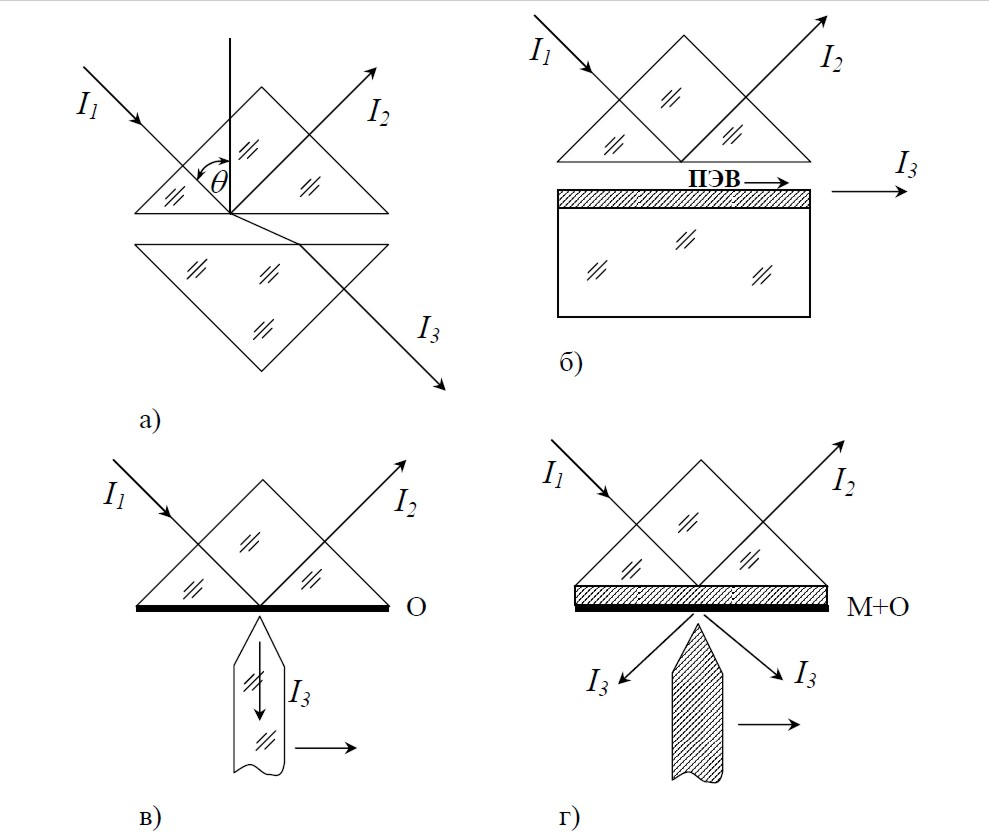
\includegraphics[width=0.9\textwidth]{schemes}
\end{center}

\column{3.5cm}

a) НПВО \\
б) Схема Кречмана \\
в) диэлектрический зонд \\
г) металлический \\ зонд

\end{columns}
\end{frame}
\section{Воздействие на частицы} 

\begin{frame}{Тензор напряжений Максвелла}

{\scriptsize
\begin{equation*}
\nabla\cdot\left[\varepsilon_0\vec  E\otimes\vec  E-\mu_0\vec  H\otimes\vec  H-\frac{1}{2}\left(\varepsilon_0E^2+\mu_0H^2\right)\hat{\vec  I}\right]=\dfrac{}{t}\frac{1}{c^2}[\vec  E\times\vec  H]+\rho\vec  E+\vec  j\times \vec  B.
\end{equation*}
\begin{multline*}
\hat{\vec  T}=\left[\varepsilon_0\vec  E\otimes\vec  E-\mu_0\vec  H\otimes\vec  H-\frac{1}{2}\left(\varepsilon_0E^2+\mu_0H^2\right)\hat{\vec  I}\right]=\\
\left[
\begin{array}{cc}
\varepsilon_0\left(E_x^2{-}\frac{E^2}{2}\right) + \mu_0\left(H_x^2{-}\frac{H^2}{2}\right)&  \varepsilon_0(E_x E_y) +\mu_0(H_x H_y) \\
\varepsilon_0(E_x E_y) + \mu_0(H_x H_y)&  \varepsilon_0\left(E_y^2{-}\frac{E^2}{2}\right) +\mu_0\left(H_y^2{-}\frac{H^2}{2}\right)\\
\varepsilon_0(E_x E_z) + \mu_0(H_x H_z)&  \varepsilon_0(E_y E_z) + \mu_0(H_y H_z)
\end{array}
\right.
\left.
\begin{array}{c}
\varepsilon_0(E_x E_z) + \mu_0(H_x H_z)\\
\varepsilon_0(E_y E_z) + \mu_0(H_y H_z)\\
\varepsilon_0\left(E_z^2{-}\frac{E^2}{2}\right)  \mu_0\left(H_z^2{-}\frac{H^2}{2}\right)
\end{array}
\right].
\end{multline*}
\begin{equation*}
\int_V\nabla\cdot\hat{\vec  T}dV=\dfrac{}{t}\frac{1}{c^2}\int_V[\vec  E\times\vec  H]dV+\int_V[\rho\vec  E+\vec  j\times\vec  B]dV.
\end{equation*}
\begin{equation*}
\boxed{
\int_{\partial V}\hat{\vec  T}(\vec  r,t)\cdot\vec  n(\vec  r) da=
\frac{d}{dt}\left(\vec  G_{\text{field}}+\vec  G_{\text{mech}}\right),
}
\end{equation*}
}
\begin{equation*}
\vec  G_{\text{field}}=\frac{1}{c^2}\int_V[\vec  E\times\vec  H]dV.
\end{equation*}
\begin{equation*}
\langle\vec  F\rangle=\int_{\partial V}\langle\hat{\vec  T}(\vec  r,t)\rangle\cdot\vec  n(\vec  r) da,
\end{equation*}

\begin{equation*}
\boxed{
\hat{\vec  T}=\left[\varepsilon_0\varepsilon\vec  E\otimes\vec  E-\mu_0\mu\vec  H\otimes\vec  H-\frac{1}{2}\left(\varepsilon_0\varepsilon E^2+\mu_0\mu H^2\right)\hat{\vec  I}\right]
}
\end{equation*}
\end{frame}


\begin{frame}{Дипольное приближение}

Если размер частиц мал по сравнению с длиной волны падающего излучения, возбуждаемый в ней отклик может быть описан как поле индуцированного диполя 

\begin{equation*}
\vec  F =\sum_i p_i \nabla E_i+\frac{d}{dt} (\vec p \times \vec B),
\end{equation*}

при усреднении по периоду осцилляций падающей волны второе слагаемое исчезает и получаем 
\begin{equation*}
\langle\vec  F \rangle= \sum_i \langle p_i(t) \nabla E_i(t) \rangle
\end{equation*}

Поляризуемость малой частицы с учетом самовоздействия
\begin{equation*}
\alpha=\frac{\alpha_0}{1-\frac{2}{3}\imath k^3\alpha_0},\quad\text{где}\quad\alpha_0 = a^3\frac{\epsilon-1}{\epsilon+1}
\end{equation*}

Таким образом, усредненная сила имеет вид:

\begin{equation*}
\boxed{
\langle\vec  F \rangle = \frac{1}{4} Re(\alpha) \nabla \left| E_0 \right|^2+\frac{1}{2} \vec k Im(\alpha) \left| E_0 \right|^2-\frac{1}{2} Im(\alpha) Im\left[\vec E_0 \cdot \nabla \vec E_0^*\right]^2
}
\end{equation*}

\end{frame}

\begin{frame}{Сила, действующая на частицу в эванесцентном поле}

Рассмотрим маленькую частицу, погруженную в эванесцентное поле, в двух поляризациях падающего поля ($k_z=\imath\sqrt{\kappa^2+k^2}$):

$TE: \vec E=(0,1,0)t_{\perp}e^{\imath \kappa x-qz}\quad TM: \vec E=(-\imath q,0,k)\frac{t_{||}}{\kappa}e^{\imath k x-qz}$, где $q=\imath k_z$

1. Компонента силы, которая связана с \textcolor{red!50!black}{градиентом} (градиентная компонента) останется только в направлении оси $z$:

\begin{equation*}
    \langle F_z\rangle=-\frac{|t|^2}{2} q Re[\alpha]e^{-2qz}=-\frac{|t|^2}{2} q \frac{Re[\alpha_0]}{4/9\kappa^6|\alpha_0|^2}e^{-2qz}
\end{equation*}

2. Компонента силы, которая связана с \textcolor{red!50!black}{рассеянием}, останется только в направлении оси $x$:

\begin{equation*}
    \langle F_x\rangle=\frac{|t|^2}{2} k Im[\alpha]e^{-2qz}=\frac{|t|^2}{2} k \frac{Im[\alpha_0]+2/3\kappa^3|\alpha_0|^2}{4/9\kappa^6|\alpha_0|^2}e^{-2qz}
\end{equation*}

\textcolor{red!50!black}{Следствие:} За исключением случаев, когда $\epsilon \in (-2,1)$, градиентная сила положительна и направлена к поверхности, рассеивающая сила всегда положительна и толкает частицу в направлении $\vec \kappa$ (В выражениях для компонент ТЕ и ТМ надо брать $t_{\perp}$ и $t_{||}$ соответственнно).

\end{frame}

\begin{frame}{Погружение  сферической частицы в эванесцентное поле}
\begin{columns}[c]

\column{9.5cm}

\begin{center}
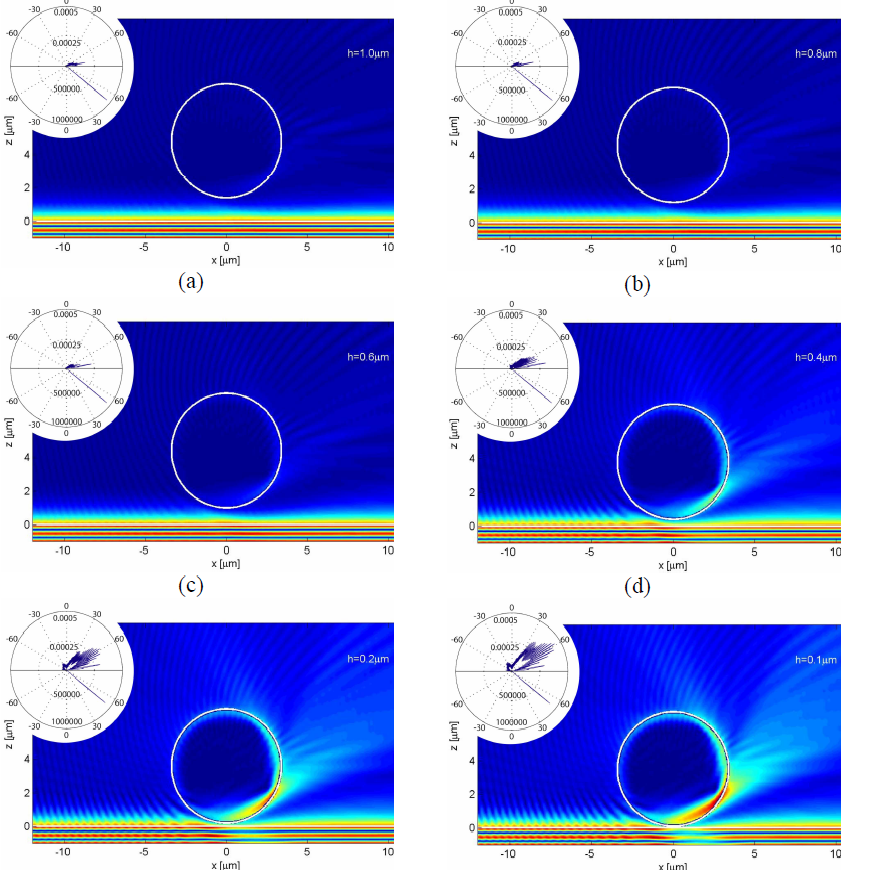
\includegraphics[width=0.85\textwidth]{lensless2}
\end{center}

\column{3cm}
$n_1=1.75$ (кварц)

$n_2=1.33$ (вода)

$n_3=1.59$ (частица)

$\lambda=1.064\quad \mu$м (Nd:YAG)

$d=6.8\quad\mu$м

$h\in (0.1-1.0)\mu$м

$\theta_1=51^{0}$

\begin{center}
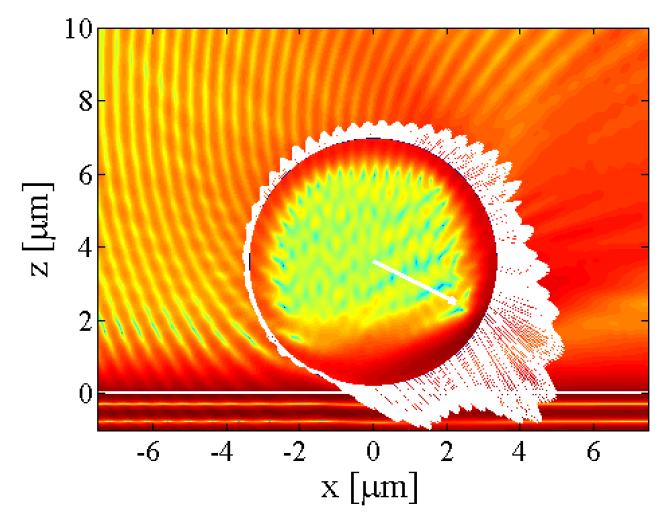
\includegraphics[width=0.95\textwidth]{lensless3}
\end{center}

\tiny{V.Ruis-Cortes, J.Vite-Frias, 2008}

\end{columns}
\end{frame}

\begin{frame}{Схема рассеяния плоской волны и эванесцентной волны}
    На основе серии работ Bekshaev-Bliokh-Nori
    
\begin{columns}[c]

\column{8cm}

\begin{center}
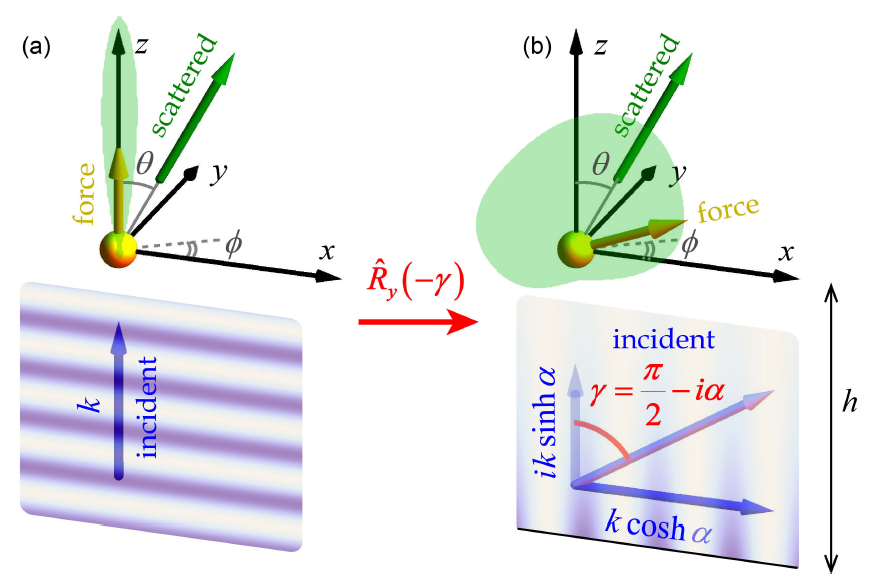
\includegraphics[width=0.9\textwidth]{bliokh0}
\end{center}

\column{4.5cm}
Если ввести оператор вращения: 
\begin{equation*}
    R_y(-\gamma)=\begin{bmatrix}
    \cos\gamma & 0 & \sin \gamma\\
    0 & 1 & 0 \\
    -\sin\gamma & 0 & \cos \gamma
    \end{bmatrix}
\end{equation*}

То при комплексном угле:

$\gamma=\frac{\pi}{2}-\imath \alpha$

получим переход от распространяющегося к эванесцентному полю

\begin{equation*}
    R_y=\begin{bmatrix}
    sinh\gamma & 0 & cosh \gamma\\
    0 & 1 & 0 \\
    -cosh\gamma & 0 & sinh \gamma
    \end{bmatrix}
\end{equation*}

\end{columns}    
    
Применяя теорию рассеяния Ми для комплексных углов:    

\small{A. Y. Bekshaev, K. Y. Bliokh, F. Nori \textbf{Mie scattering and optical forces from evanescent fields: а complex-angle approach} (2013)}
\end{frame}



\begin{frame}{Рассеяние Ми в плоских и эванесцентных полях: S-поляризация}
Индикатриссы рассеяния в дальнем поле для частиц разного размера.
\begin{center}
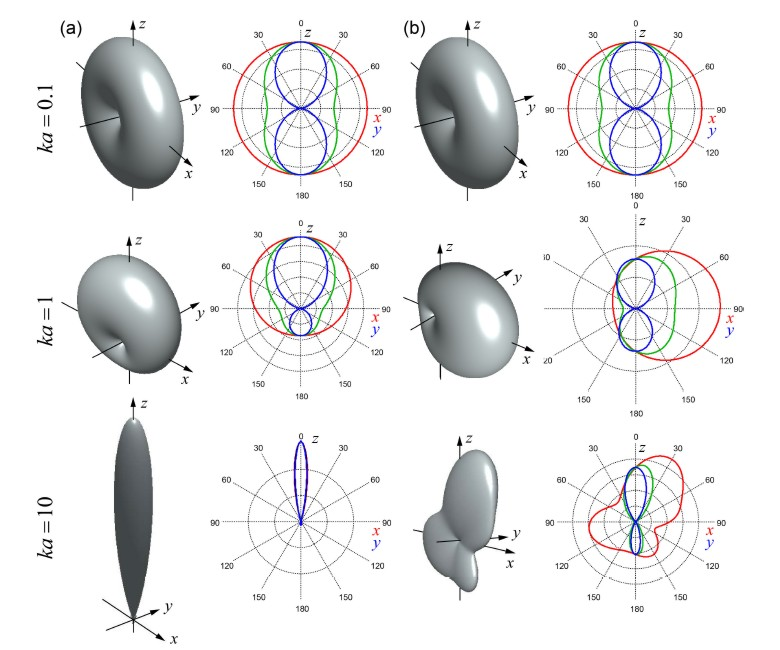
\includegraphics[width=0.7\textwidth]{mie1}
\end{center}

Слева: Стандартная теория рассеяния Ми плоской волны.

Справа: Теория Ми для комплексного угла.
\end{frame}

\begin{frame}{Рассеяние Ми в плоских и эванесцентных полях: P-поляризация}

\begin{center}
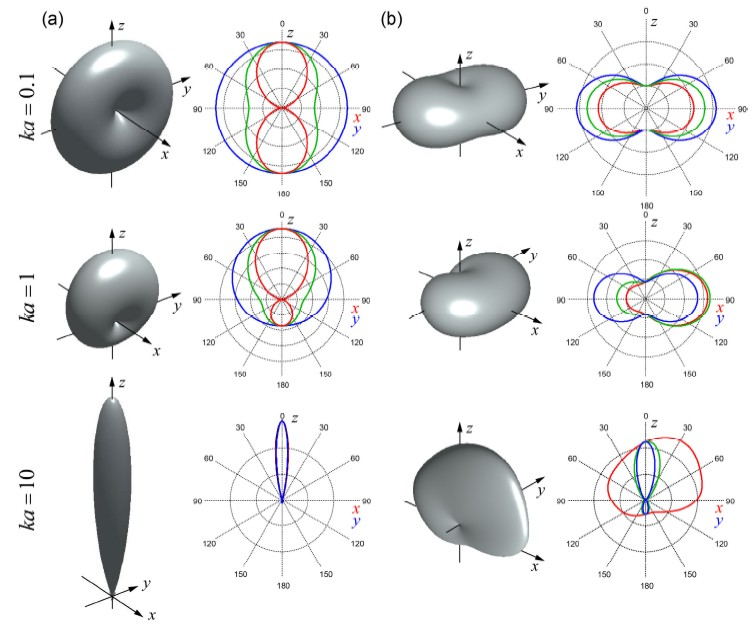
\includegraphics[width=0.7\textwidth]{mie2}
\end{center}
 То же для P-поляризации.

\textcolor{red!50!black}{Важно:} при решении этой задачи не учитывалось влияние поверхности, без которой невозможно существование эванесцентного поля.
\end{frame}

\begin{frame}{Силы, действующие вдоль и поперек направления распространения}

\begin{center}
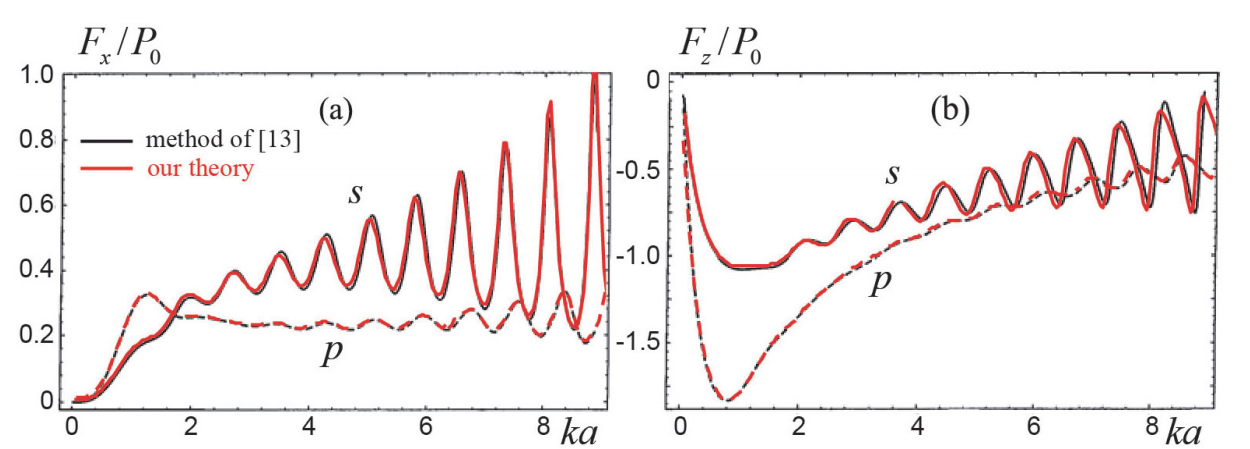
\includegraphics[width=0.95\textwidth]{bliokh4}
\end{center}

Видим наличие характерных форм-факторных резонансов Ми. 

Отличие $F_z$ от $F_x$  в том, что ее величина (в области до резонансов) по модулю сначала уменьшается, затем увеличивается.

Учет влияния поверхности становится довольно сложной задачей с точки зрения теоретического описания: см. L.Novotny, B.Hecht, Ch. 10 Dipole emission near planar interface, p.313.

\end{frame}

\begin{frame}{Средняя сила и ее компоненты в случае металлической частицы}

Влияние приближения к плазмонному резонансу:

\begin{center}
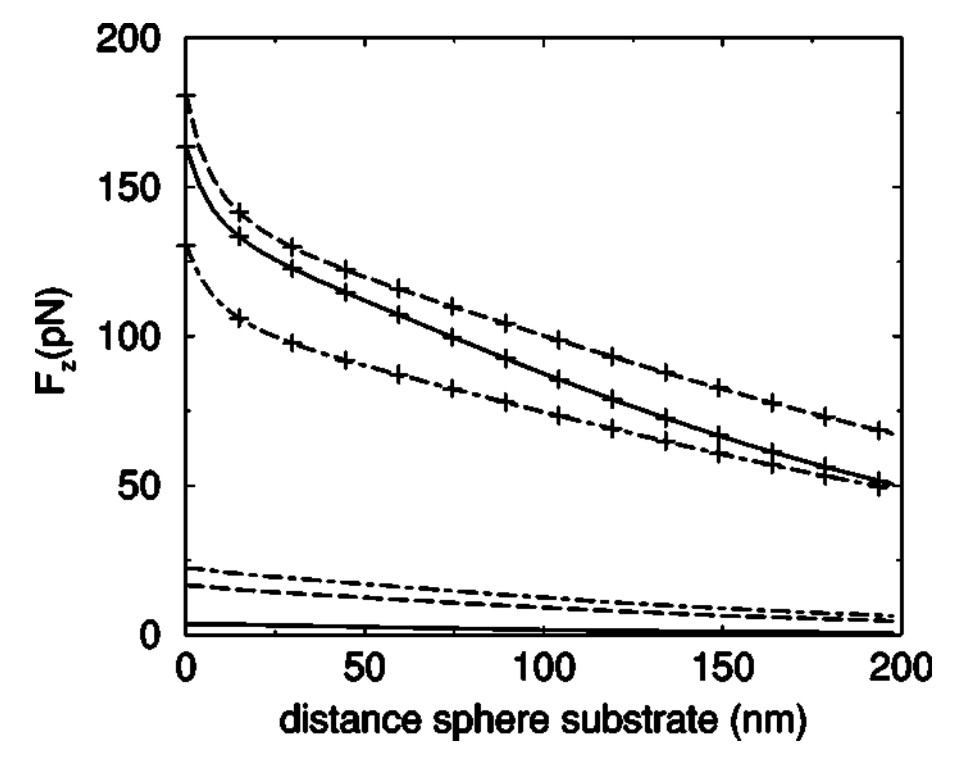
\includegraphics[width=0.65\textwidth]{force}
\end{center}

\small{Серебряная (сплошная,  $\lambda=480$ нм), золотая (пунктирная, $\lambda=640$ нм), медная (штрих-пунктирная, $\lambda=605$ нм) в резонансе}

\small{Серебряная (сплошная,  $\lambda=400$ нм), золотая (пунктирная, $\lambda=400$ нм), медная (штрих-пунктирная, $\lambda=300$ нм) вне резонанса}

\end{frame}


\begin{frame}{Средняя сила и ее компоненты для двух стеклянных шариков}
\begin{columns}
\column{6.5cm}

\begin{center}
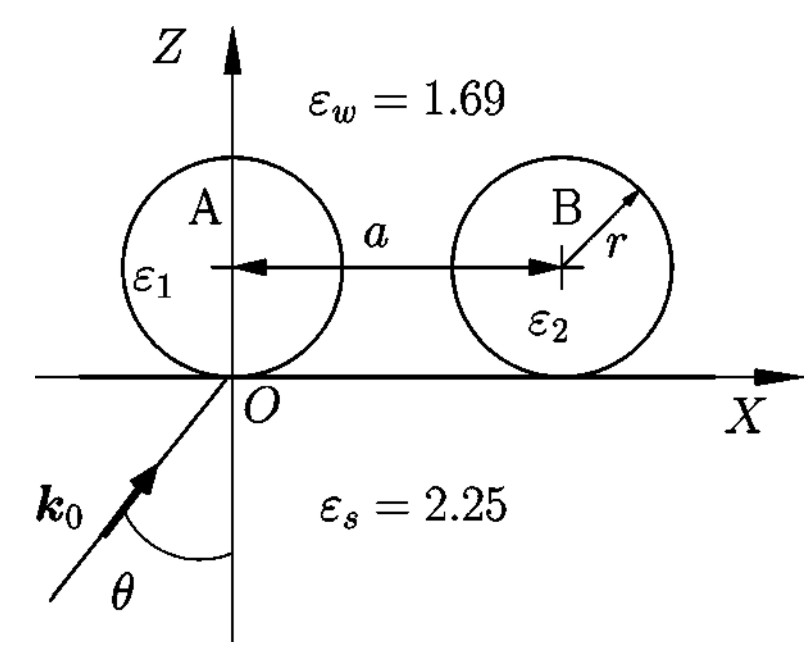
\includegraphics[width=1\textwidth]{spheres}
\end{center}

\column{6.5cm}

\begin{center}
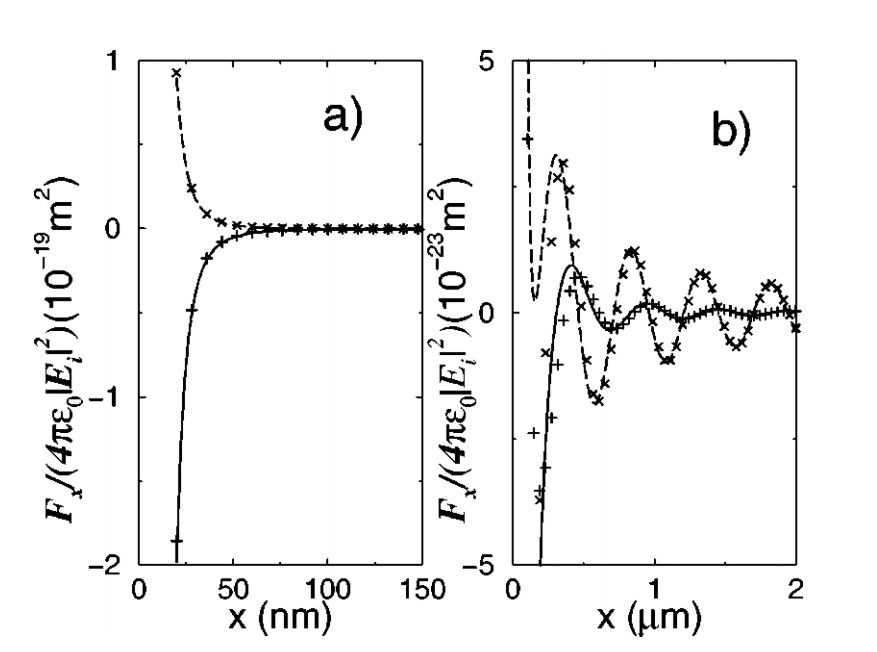
\includegraphics[width=1\textwidth]{force_two_spheres}
\end{center}

\end{columns}

Сила, действующая на левый шарик, для случая, когда шарики находятся в ближем поле друг друга (слева) и дальнем (справа)
\end{frame}

\begin{frame}{Вращающий момент, действующий на частиу в эванесцентном поле}
\begin{center}
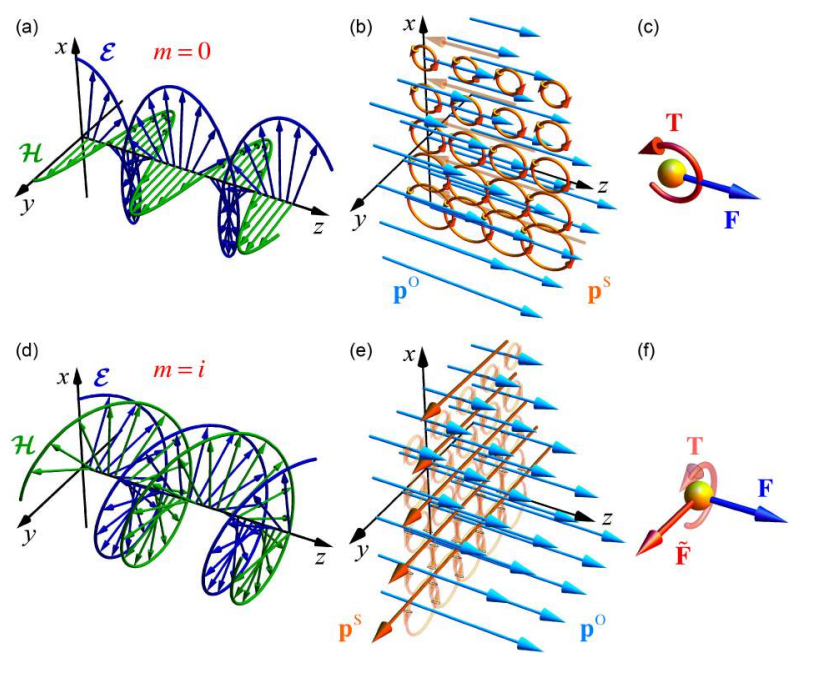
\includegraphics[width=0.8\textwidth]{bliokh6}
\end{center}
\end{frame}

\begin{frame}{Вращающий момент, действующий на частиу в эванесцентном поле}
\begin{center}
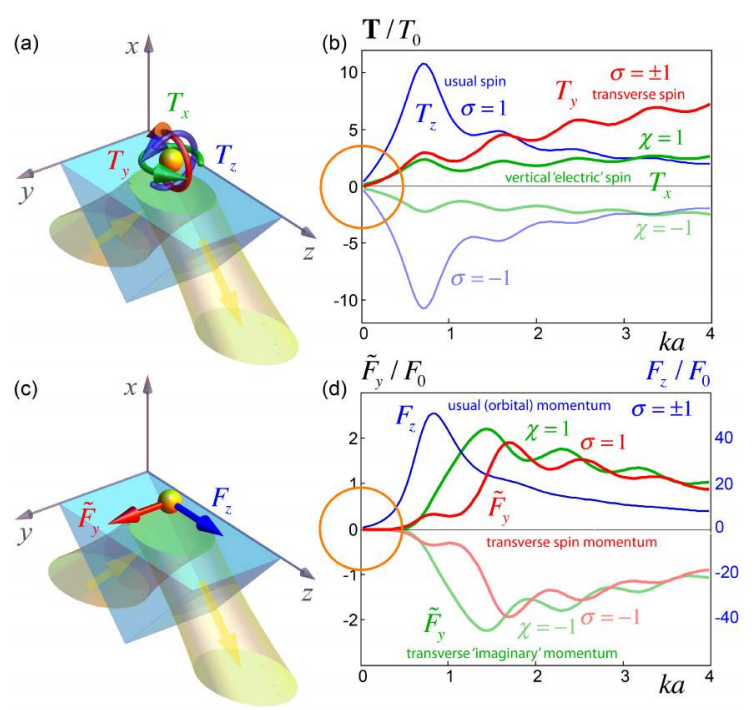
\includegraphics[width=0.8\textwidth]{bliokh7}
\end{center}
\end{frame}
\section{Поляризационные свойства} 


\begin{frame}{Распределение поляризации ближнего поля}
\begin{columns}
\column{5cm}
\begin{equation*}
E_x(\vec r,t)=A_x(\vec r)\cos(\omega t + \phi_x(\vec  r))
\end{equation*}
\begin{equation*}
E_y(\vec r,t)=A_y(\vec r)\cos(\omega t + \phi_y(\vec  r))
\end{equation*}
\begin{equation*}
E_z(\vec r,t)=A_z(\vec r)\cos(\omega t + \phi_z(\vec  r))
\end{equation*}
\column{7cm}

Параметры Стокса:
\begin{equation*}
S_{3xy}=\imath(\langle E_x^*(\vec r, \omega) E_y(\vec r, \omega)\rangle-\langle E_x(\vec r, \omega) E_y^*(\vec r, \omega)\rangle )
\end{equation*}
\begin{equation*}
S_{3xz}=\imath(\langle E_x^*(\vec r, \omega) E_z(\vec r, \omega)\rangle-\langle E_x(\vec r, \omega) E_z^*(\vec r, \omega)\rangle )
\end{equation*}
\begin{equation*}
S_{3yz}=\imath(\langle E_y^*(\vec r, \omega) E_z(\vec r, \omega)\rangle-\langle E_y(\vec r, \omega) E_z^*(\vec r, \omega)\rangle )
\end{equation*}
\end{columns}
\begin{center}
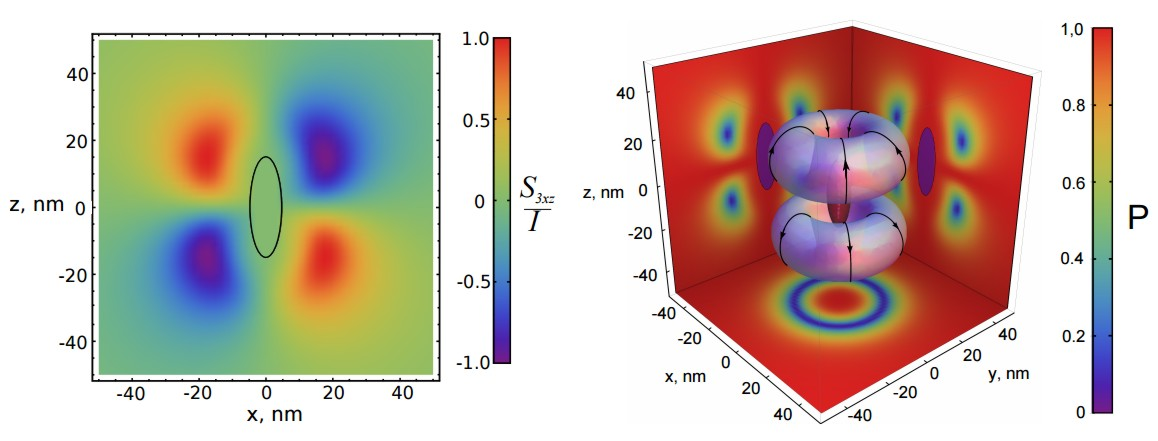
\includegraphics[width=0.8\textwidth]{polar}
\end{center}

Поляризация ближнего поля вытянутого эллипсоида вблизи его плазмонного резонанса. Падающее поле линейно поляризовано вдоль оси z.

\scriptsize{V.N.Zadkov, OPTICS EXPRESS, 2014}

\end{frame}



\end{document}

